% !TeX spellcheck = en_US
\tikzset{
	operation/.style={fill=white, text centered},
	block/.style = {operation, rectangle, draw, text width=0.175\textwidth, minimum height=1cm},
}
\begin{tikzpicture}[node distance = 1cm and 1.75cm]
	\node (image)           [block] {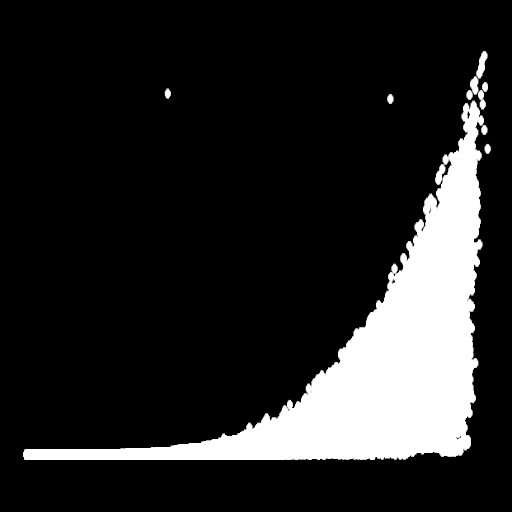
\includegraphics[width=\textwidth]{figures/input.jpg} Image \image};
	\node (aperture)        [block, right = of image] {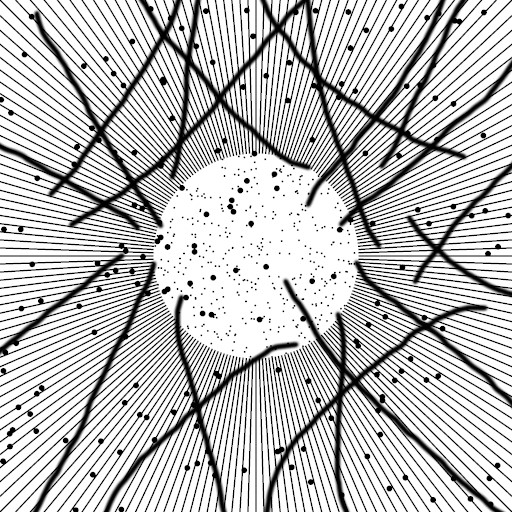
\includegraphics[width=\textwidth]{figures/aperture.jpg} Aperture \aperture};
	\node (blobMask)        [block, below = of image] {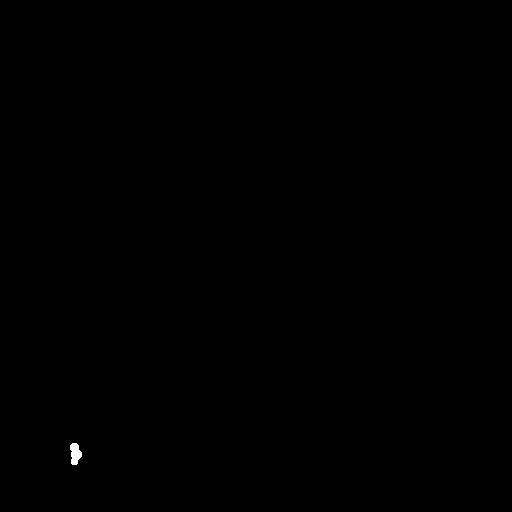
\includegraphics[width=\textwidth]{figures/blobMask.jpg} Blob mask \blobmask};
	\node (tonemappedImage) [block, left = of blobMask] {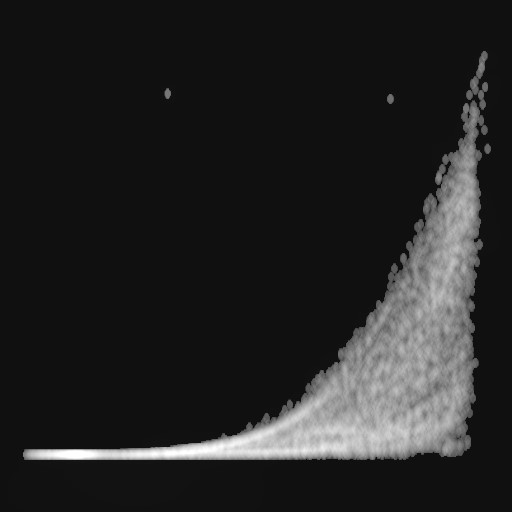
\includegraphics[width=\textwidth]{figures/tonemappedImage.jpg} Tone mapped image \tonemappedimage};
	\node (overlay)         [block, below = of blobMask] {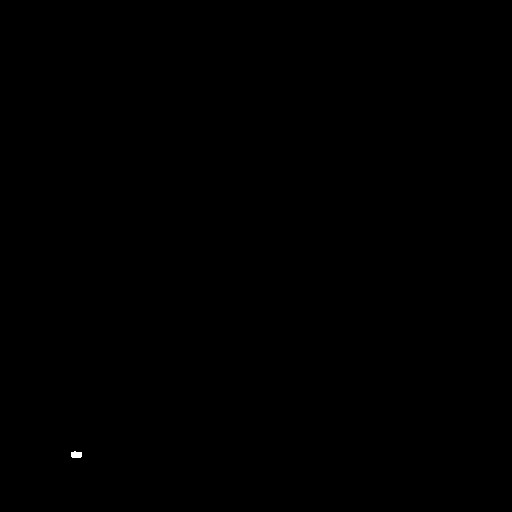
\includegraphics[width=\textwidth]{figures/overlay.jpg} Bright pixels \overlay};
	\node (psf)             [block, right = of overlay] {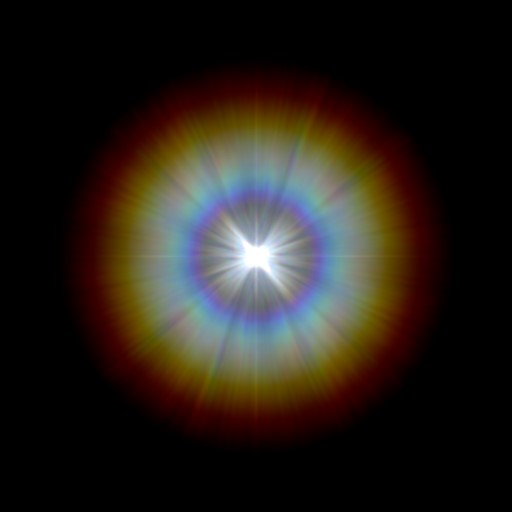
\includegraphics[width=\textwidth]{figures/psf.jpg} Glare filter \psf};
	\node (glareOverlay)    [block, below = of overlay] {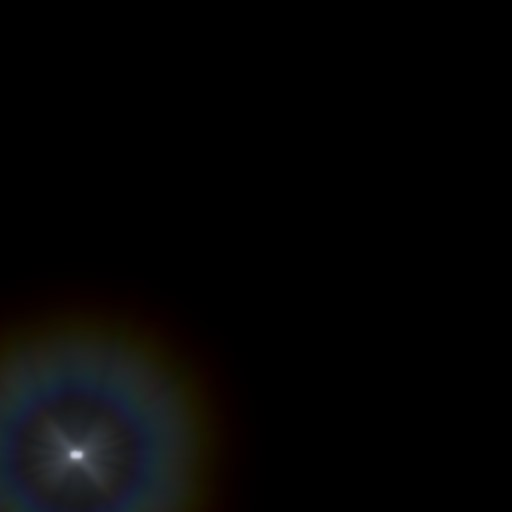
\includegraphics[width=\textwidth]{figures/glareOverlay.jpg} Glare overlay \glareoverlay};
	\node (output)          [block, below = of glareOverlay] {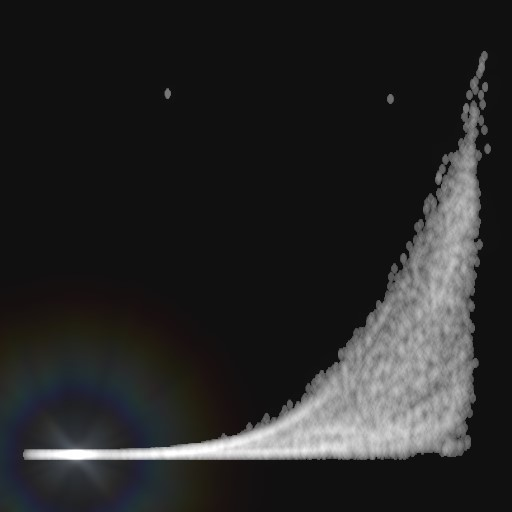
\includegraphics[width=\textwidth]{figures/output.jpg} Tone mapped and glared image \finalimage};
	
	\draw[white] (image) -- node(dummy){} (aperture);
	
	\draw[->] (image) -- node(detection)[operation]{Blob detection} (blobMask);
	\draw[->] (image) -| node[operation]{Tone mapping} (tonemappedImage);
	\draw[->] (aperture) -- node[operation, text width = 0.175\textwidth]{Diffraction approximation} (psf);
	
	\draw[->] (blobMask) -- node(masking)[operation]{Masking} (overlay);
	\draw     (tonemappedImage) |- (masking);
	\draw     (image) -- (dummy.center) |- (masking);
	
	\draw[->] (overlay) -- node(convolution)[operation]{Convolution} (glareOverlay);
	\draw     (psf) |- (convolution);
	
	\draw[->] (glareOverlay) -- node(adding)[operation]{Blending} (output);
	\draw     (tonemappedImage) |- (adding);
\end{tikzpicture}